\documentclass[12pt]{article}
\usepackage[utf8]{inputenc}

%allows you to neatly integrate an abstract once you start with the actual content
\usepackage{abstract}
\usepackage{microtype}
\usepackage{enumitem}

%%%%%%%%%%%%%%%%%%%%%%%%%%%%%%%%%%%%%%%%%%%%%%%%%%%%%%%%%%%%%%%%%%%%%%%%%%%%%%%%%%%%%%%%%% 
% SETTING THE GEOMETRY
%%%%%%%%%%%%%%%%%%%%%%%%%%%%%%%%%%%%%%%%%%%%%%%%%%%%%%%%%%%%%%%%%%%%%%%%%%%%%%%%%%%%%%%%%%

%borders and such
\usepackage
[
margin=1.5in
%a4paper,% other options: a3paper, a5paper, etc
%left=2.5cm,
%right=2.5cm, top=5cm,
% use vmargin=2cm to make vertical margins equal to 2cm.
% us  hmargin=3cm to make horizontal margins equal to 3cm.
% use margin=3cm to make all margins  equal to 3cm.
]
{geometry}
%makes for onehalfspacing in the whole document
\usepackage{setspace} 
\onehalfspacing
% \doublespacing
% allows to enter other margins for big figures or tables
\usepackage{changepage}
% disallow footnotes to extend over more than one page
\interfootnotelinepenalty=10000

%%%%%%%%%%%%%%%%%%%%%%%%%%%%%%%%%%%%%%%%%%%%%%%%%%%%%%%%%%%%%%%%%%%%%%%%%%%%%%%%%%%%%%%%%% 
% FONTS & COLORS
%%%%%%%%%%%%%%%%%%%%%%%%%%%%%%%%%%%%%%%%%%%%%%%%%%%%%%%%%%%%%%%%%%%%%%%%%%%%%%%%%%%%%%%%%% 
% Obviously colors. Usage: \color{red} Red text. This also allows you to make custom colors
\usepackage{xcolor}      
%if you want to start a multicolomns part inside your normally one columned article
\usepackage{multicol}
%titlesec allows you to change the way, titles are presented in latex
% \usepackage{titlesec}
%lets you change the style of your (sub)section headers
\usepackage{sectsty}
%I chose to make my headers cyan-colored
\sectionfont{\fontsize{16}{15}\selectfont}
\subsectionfont{\fontsize{14}{15}\selectfont}
\subsubsectionfont{\fontsize{12}{15}\selectfont}
% \subsectionfont{\color{cyan}}
% \subsubsectionfont{\color{cyan}}  
% \paragraphfont{\color{cyan}} 

% superscript 1st, 2nd, 3rd, 4th ... use \nth{8}
\usepackage[super]{nth}

%%%%%%%%%%%%%%%%%%%%%%%%%%%%%%%%%%%%%%%%%%%%%%%%%%%%%%%%%%%%%%%%%%%%%%%%%%%%%%%%%%%%%%%%%% 
% CITATION
%%%%%%%%%%%%%%%%%%%%%%%%%%%%%%%%%%%%%%%%%%%%%%%%%%%%%%%%%%%%%%%%%%%%%%%%%%%%%%%%%%%%%%%%%% 

\usepackage[english]{babel}
\usepackage{csquotes}

\usepackage[authordate,backend=biber,uniquename=false,uniquelist=false]{biblatex-chicago}
\bibliography{references}

\ExecuteBibliographyOptions{
    giveninits=true,
    % isbn=false,
    url=true,
    doi=true,
    % uniquename=init
    }
    
\DeclareBibliographyAlias{webpage}{online} 
\AtEveryBibitem{\clearlist{language}}
\AtEveryBibitem{%
      \ifentrytype{online}
        {}
        {\clearfield{urlyear}\clearfield{urlmonth}\clearfield{urlday}}
    }

%%%%%%%%%%%%%%%%%%%%%%%%%%%%%%%%%%%%%%%%%%%%%%%%%%%%%%%%%%%%%%%%%%%%%%%%%%%%%%%%%%%%%%%%%% 
% INSERTING PICTURES
%%%%%%%%%%%%%%%%%%%%%%%%%%%%%%%%%%%%%%%%%%%%%%%%%%%%%%%%%%%%%%%%%%%%%%%%%%%%%%%%%%%%%%%%%% 

%very useful if you want to add a jpfg or png file. Usage: \includegraphics{path/to/file}
\usepackage{grffile}
\usepackage{graphicx}
\usepackage{subcaption}
\usepackage[format=plain,
            % labelfont=it,
            font=footnotesize,
            % width=0.85\textwidth,
            % textfont=it,
            % singlelinecheck=on
            ]{caption}
% Figures can't live outside the section
\usepackage[section]{placeins}
% and then also \FloatBarrier at the end of a section to enforce harder.

% For figures turned 90 degrees
\usepackage{rotating}
% For uppercase subfigure panels
\renewcommand{\thesubfigure}{\Alph{subfigure}}


% Draw pictures, like game trees
\usepackage{tikz}
\usetikzlibrary{trees}
% Node styles
\tikzset{
% Two node styles for game trees: solid and hollow
solid node/.style={circle,draw,inner sep=1.5,fill=black},
hollow node/.style={circle,draw,inner sep=1.5,fill=white}
}
\usepackage{pgfplots}
\usepgfplotslibrary{fillbetween}


%%%%%%%%%%%%%%%%%%%%%%%%%%%%%%%%%%%%%%%%%%%%%%%%%%%%%%%%%%%%%%%%%%%%%%%%%%%%%%%%%%%%%%%%%% 
% INSERTING TABLES
%%%%%%%%%%%%%%%%%%%%%%%%%%%%%%%%%%%%%%%%%%%%%%%%%%%%%%%%%%%%%%%%%%%%%%%%%%%%%%%%%%%%%%%%%% 

\usepackage{array}
\usepackage{tabularx}
\usepackage{longtable}
\newcolumntype{x}[1]{>{\let\newline\\\arraybackslash\hspace{0pt}}p{#1}}
\newcolumntype{y}[1]{>{\centering\let\newline\\\arraybackslash\hspace{0pt}}p{#1}}
\newcolumntype{s}[1]{>{\centering\arraybackslash}p{#1}}
\renewcommand*{\arraystretch}{1.2}

\usepackage{multirow}

%%%%%%%%%%%%%%%%%%%%%%%%%%%%%%%%%%%%%%%%%%%%%%%%%%%%%%%%%%%%%%%%%%%%%%%%%%%%%%%%%%%%%%%%%% 
% LINKS AND WWW
%%%%%%%%%%%%%%%%%%%%%%%%%%%%%%%%%%%%%%%%%%%%%%%%%%%%%%%%%%%%%%%%%%%%%%%%%%%%%%%%%%%%%%%%%% 

% Provides clickable links in the PDF-document for \ref and the TOC
\usepackage[hidelinks]{hyperref} %you can remove the hidelinks option to make the hyperrefs visible. looks very ugly to me, but might be useful to less experienced readers of pdfs
% Lets you typeset urls with linebreak. Usage: \url{http://...}  
\usepackage{url}

%%%%%%%%%%%%%%%%%%%%%%%%%%%%%%%%%%%%%%%%%%%%%%%%%%%%%%%%%%%%%%%%%%%%%%%%%%%%%%%%%%%%%%%%%% 
% CODE INTEGRATION
%%%%%%%%%%%%%%%%%%%%%%%%%%%%%%%%%%%%%%%%%%%%%%%%%%%%%%%%%%%%%%%%%%%%%%%%%%%%%%%%%%%%%%%%%% 

% Source Code Listings. Usage: \begin{lstlisting}...\end{lstlisting}
\usepackage{listings}
%this defines a lot of parameters for code. makes it look nice IMO
\lstset{ 
	breaklines=true,                 % sets automatic line breaking
	commentstyle=\color{mygreen},    % comment style
	escapeinside={\%*}{*)},          % if you want to add LaTeX within your code
	frame=single,	                   % adds a frame around the code
	keepspaces=true,                 % keeps spaces in text, useful for keeping indentation of code (possibly needs columns=flexible)
	keywordstyle=\color{blue},       % keyword style
	numbers=left,                    % where to put the line-numbers; possible values are (none, left, right)
	numbersep=5pt,                   % how far the line-numbers are from the code
	numberstyle=\tiny\color{mygray}, % the style that is used for the line-numbers
	rulecolor=\color{black},         % if not set, the frame-color may be changed on line-breaks within not-black text (e.g. comments (green here))
	showspaces=false,                % show spaces everywhere adding particular underscores; it overrides 'showstringspaces'
	showstringspaces=false,          % underline spaces within strings only
	showtabs=false,                  % show tabs within strings adding particular underscores
	stepnumber=2,                    % the step between two line-numbers. If it's 1, each line will be numbered
	stringstyle=\color{mymauve},     % string literal style
	tabsize=2,	                   % sets default tabsize to 2 spaces
	title=\lstname                   % show the filename of files included with \lstinputlisting; also try caption instead of title
}         

%%%%%%%%%%%%%%%%%%%%%%%%%%%%%%%%%%%%%%%%%%%%%%%%%%%%%%%%%%%%%%%%%%%%%%%%%%%%%%%%%%%%%%%%%% 
% MATH
%%%%%%%%%%%%%%%%%%%%%%%%%%%%%%%%%%%%%%%%%%%%%%%%%%%%%%%%%%%%%%%%%%%%%%%%%%%%%%%%%%%%%%%%%% 

%some very useful packages for writing down beautiful formulas
\usepackage{amsmath}
\usepackage{amssymb}
\usepackage{mathtools}
\usepackage{mathrsfs}  
\usepackage{bm}
\usepackage{empheq}
% Nice rules for tables. Usage \begin{tabular}\toprule ... \midrule ... \bottomrule
\usepackage{booktabs}          

%%%%%%%%%%%%%%%%%%%%%%%%%%%%%%%%%%%%%%%%%%%%%%%%%%%%%%%%%%%%%%%%%%%%%%%%%%%%%%%%%%%%%%%%%% 
% APPENDIX
%%%%%%%%%%%%%%%%%%%%%%%%%%%%%%%%%%%%%%%%%%%%%%%%%%%%%%%%%%%%%%%%%%%%%%%%%%%%%%%%%%%%%%%%%% 

\usepackage{appendix}
% Change numbering of figures, tabels etc. in Appendix
\usepackage{chngcntr} 

\usepackage{titletoc}


%%%%%%%%%%%%%%%%%%%%%%%%%%%%%%%%%%%%%%%%%%%%%%%%%%%%%%%%%%%%%%%%%%%%%%%%%%%%%%%%%%%%%%%%%% 
% ALL ABOUT YOU
%%%%%%%%%%%%%%%%%%%%%%%%%%%%%%%%%%%%%%%%%%%%%%%%%%%%%%%%%%%%%%%%%%%%%%%%%%%%%%%%%%%%%%%%%% 


\title{22BDP Microeconomics week 4}
\author{Tom Rodriguez, Bénédicte Droz}
\date{06.08.2023}

%start your document with \begin{document} and type everything inbetween \begin{document} and \end{document}
\begin{document}

\begin{titlepage}
	
	\newcommand{\HRule}{\rule{\linewidth}{0.5mm}} % Defines a new command for the horizontal lines, change thickness here
	
	\center % Center everything on the page
	
	%----------------------------------------------------------------------------------------
	%	HEADING SECTIONS
	%----------------------------------------------------------------------------------------
	
% 	\includegraphics{Figures/UZH.eps} \\[1.5cm] 
    %	\textsc{\LARGE University of Zurich}\\[1.5cm] % Name of your university/college and the size of the distance to the next line. \LARGE is used to make really big fonts
	\textsc{\large Beginning Doctoral Program Gerzensee}\\[0.5cm] % Major heading such as course name
	{\large Lectures held by Klaus Schmidt and Piero Gottardi}\\[1cm] % you can the name(s) of your instructor(s)
	
	
	%----------------------------------------------------------------------------------------
	%	TITLE SECTION
	%----------------------------------------------------------------------------------------
	
	\HRule \\[1.0cm]
	{ \LARGE \bfseries Microeconomics Midterm Solutions}\\[0.4cm] % Title of your document, and yes, I am aware that it is stupid to have to list it twice. I don't know how to work around this.
	\HRule \\[2cm]
	
	%----------------------------------------------------------------------------------------
	%	AUTHOR SECTION
	%----------------------------------------------------------------------------------------
	

	
	\begin{flushleft}
        \Large List of Contributors:
        
        \color{blue}
		{\large 
            \href{https://rodrigueztom.github.io}{Tom Rodriguez (University of Fribourg)}
        }\color{black}
	\end{flushleft}
	
	
	%----------------------------------------------------------------------------------------
	%	DATE SECTION
	%----------------------------------------------------------------------------------------
	
	{\large \today} % Date, change the \today to a set date if you want to be precise
	
	% Fill the rest of the page with whitespace
	\vfill 
	
\end{titlepage}

%%%%%%%%%%%%%%%%%%%%%%%%%%%%%%%%%%%%%%%%%%%%%%%%%%%%%%%%%%%%%%%%%%%%%%%%%%%%%%%%%%%%%%%%%% 
% GEOMETRY according to university guidelines
%%%%%%%%%%%%%%%%%%%%%%%%%%%%%%%%%%%%%%%%%%%%%%%%%%%%%%%%%%%%%%%%%%%%%%%%%%%%%%%%%%%%%%%%%% 

%This line can be used to adjust the geometry of the document according to the university guidelines for borders and such
% \newgeometry{margin=1.5in}

%%%%%%%%%%%%%%%%%%%%%%%%%%%%%%%%%%%%%%%%%%%%%%%%%%%%%%%%%%%%%%%%%%%%%%%%%%%%%%%%%%%%%%%%%% 
% ABSTRACT
%%%%%%%%%%%%%%%%%%%%%%%%%%%%%%%%%%%%%%%%%%%%%%%%%%%%%%%%%%%%%%%%%%%%%%%%%%%%%%%%%%%%%%%%%% 

%\thispagestyle{empty} %suppresses the footer and header since I want to start show them after the TOC, optional
\pagenumbering{roman}	
% \tableofcontents

% The \clearpage command is a pagebreak to separate the abstract from the content
%\clearpage
\newpage
\pagenumbering{arabic}

%%%%%%%%%%%%%%%%%%%%%%%%%%%%%%%%%%%%%%%%%%%%%%%%%%%%%%%%%%%%%%%%%%%%%%%%%%%%%%%%%%%%%%%%%% 
 % ACTUAL CONTENT 
%%%%%%%%%%%%%%%%%%%%%%%%%%%%%%%%%%%%%%%%%%%%%%%%%%%%%%%%%%%%%%%%%%%%%%%%%%%%%%%%%%%%%%%%%%

\newpage
\section*{Microeconomics Midterm 2011 / 12}

{
\subsection*{Schmidt}

\subsubsection*{Exercise 1}

\begin{enumerate}[label=(\alph*)]
{\item 
Yes since

\begin{align*}
    x_k(\lambda p, \lambda w) & =\frac{\lambda w}{\sum_{e=1}^c \lambda p_e}=\frac{\lambda}{\lambda} \frac{w}{\sum_{l=1}^{\infty} p_e} \\
    & =\frac{w}{\sum_{e=1}^l p_e}=x_k(p, w)
\end{align*}
}
{\item 
Yes since

\begin{align*}
\begin{aligned}
    \sum_{k=1}^L x_k p_k & =\sum_{k=1}^L \frac{w}{\sum_{\ell=1}^w p_e} p_k=\frac{w}{\sum_{\ell=1}^L p_e} \sum_{k=1}^L p_k \\
    & =w \frac{\sum_{k=1}^L p_k}{\sum_{\ell=1}^L p_e}=w
\end{aligned}
\end{align*}
}
{\item 
Yes since WA says that

\begin{align*}
    p \times\left(p^{\prime}, w^{\prime}\right) \leqslant w \Longrightarrow p^{\prime} \times(p, w)>w^{\prime}
\end{align*}

In our case:

\begin{align*}
    \underbrace{w^{\prime} \frac{\sum_{\ell=1}^L p_l}{\sum_{\ell=1}^L p_l^{\prime}} \leqslant w}_{\text {(I) }} \Rightarrow \underbrace{w \frac{\sum_{\ell=1}^L p_e^{\prime}}{\sum_{\ell=1}^L p_e}>w^{\prime}}_{\text {(II) }}
\end{align*}

From (I) and $x(p, w) \neq x\left(p^{\prime}, w^{\prime}\right)$ implies (II). Thus, WA is satisfied!
}
{\item 
\begin{align*}
    s_{l k}(p, w) & =\frac{\partial x_k(p, w)}{\partial p_k}+\frac{\partial x_l(p, w)}{\partial w} x_k(p, w) \\
    & =-\frac{w}{\left(\sum_{l=1}^L p_l\right)^2}+\frac{w}{\left(\sum_{l=1}^L p_l\right)^2}=0
\end{align*}

Since all entries are zero it is symmetric and negative semidefinite.
}
\end{enumerate}

\subsubsection*{Exercise 2}

\begin{enumerate}[label=(\alph*)]
{\item 
This is immediate. Since preferences are represented by $f(x)=g(h(x))$, they are also represented by $h(x)$ as utility is only ordinal.

\begin{align*}
    x>y &\Longleftrightarrow f(x)>f(y) \quad \text{by utility function} \\
    f(x)>f(y) &\Longleftrightarrow h(x)>h(y) \quad \text{by monotonic transformation}
\end{align*}
}
{\item 
$e(p, u)$ is the answer to

\begin{align*}
    \min_x p x \text{ s.t. } u(x)=u
\end{align*}


(1) Let $u(x)=1$, and $x^*$ the solution: 

\begin{align*}
    &\min_x p x \text{ s.t. } u(x)=1 \\
    &\longrightarrow x^*=\operatorname{argmin}(p x) \\
    &\longrightarrow u\left(x^*\right)=1
\end{align*}
}
\end{enumerate}
}

{
\subsection*{Gottardi}

\subsubsection*{Exercise 1}

\begin{enumerate}[label=(\alph*)]
{\item 
\underline{Agent h:} 

\begin{align*}
    & \max _{x^h} \ln \left(x_1^h\right)+k^h \ln \left(x_2^h\right) \\
    & \text { s.t. } p x_1^h+x_2^h=p w_1^h+w_2^h
\end{align*}

First order conditions:

\begin{align*}
    \frac{1}{x^\mu}-\lambda p &= 0 \\
    \frac{k^n}{x_2^h}-\lambda &= 0 \\
    \Rightarrow x_2^h &= k^h p x_1^h \tag{1}
\end{align*}

Plug (1) into $B C$ for $A$:

\begin{align*}
p x_1^A+3 p x_1^A=p 13 \Longleftrightarrow x_1^A=\frac{13}{4}
\end{align*}

Plug (1) into $B C$ for $B$:

\begin{align*}
p x_1^B+p x_1^B=14 \Longleftrightarrow x_1^3=\frac{7}{p}
\end{align*}

\underline{Market clearing:}

\begin{align*}
    x_1^B=13-x_1^A=\frac{3.13}{4}=\frac{39}{4} \rightarrow \frac{39}{4}&=\frac{7}{p} \\
    \Longleftrightarrow p=\frac{4\cdot7}{39}&=\frac{28}{39} \\
    x_2^A=3 \cdot p \cdot x_1^A=3 \frac{28}{35} \frac{13}{4}=\frac{7 \cdot 13}{13}&=7 \\
    x_2^B&=7
\end{align*}

\underline{Competitive Equilibrium:}

\begin{align*}
    \left(x_1^A, x_2^A\right)&=(\frac{13}{4},7) \\
    \left(x_1^B, x_2^B\right)&=(\frac{39}{4},7) \\
    p &= \frac{28}{39}
\end{align*}
}
{\item 
Yes. 

\begin{align*}
    M R S^A &= \frac{x_2^A}{3 x_1^A}=\frac{7}{3\cdot \frac{13}{4}}=\frac{28}{39} \\
    M R S^B &= \frac{x_2^B}{x_1^B}=\frac{7}{\frac{39}{4}}=\frac{28}{39}
\end{align*}

Also: markets are complete, there's free disposal, and LNS is satisfied.
}
{\item 
Yes. 

\begin{align*}
    \operatorname{MRS}^A(4,8) &= \frac{8}{3 \cdot 4}=\frac{2}{3} \\
    \operatorname{MRS}^B(9,6) &= \frac{6}{9}=\frac{2}{3}
\end{align*}

As preferences are convex, we can decentralize:

\begin{align*}
& T^A=\left[\begin{array}{l}
x_1^A-w_1^A \\
x_2^A-w_2^A
\end{array}\right]=\left[\begin{array}{c}
4-13 \\
8
\end{array}\right]=\left[\begin{array}{c}
-9 \\
8
\end{array}\right] \\
& T^B=\left[\begin{array}{l}
x_1^B-w_1^B \\
x_2^B-w_2^B
\end{array}\right]=\left[\begin{array}{c}
9 \\
6-14
\end{array}\right]=\left[\begin{array}{c}
9 \\
-8
\end{array}\right]
\end{align*}

At equilibrium, relative price must be equal to MRS. Thus $p=\frac{2}{3}$.
}
\end{enumerate}

\subsubsection*{Exercise 2}

\begin{enumerate}[label=(\alph*)]
{\item
at $t=0: \quad\quad\quad\quad q_1 \theta_1+c_2 \theta_2=0$ 

at $t=0: s=1: \quad x_1=w_1+3 \theta_1+\theta_2=10+3 \theta_1+\theta_2$

at $t=0: s=2: \quad x_2=w_2+ \theta_1+3\theta_2=4+\theta_1+3\theta_2$
}
{\item
We solve the consumer problem:

\begin{align*}
    \max _x \frac{1}{2}\left[\ln \left(x_1\right)+\ln \left(x_2\right)\right] \text { s.t. BCs from (a) }
\end{align*}

substitute $(x_1, x_2)$ from the BC in (a):

\begin{align*}
    &\max _\theta \frac{1}{2}\left[\ln \left(10+3 \theta_1+\theta_2\right)+\ln \left(4+\theta_1+3 \theta_2\right)\right] \\
    &\text { s.t. } q_1 \theta_1+q_2 \theta_2=0
\end{align*}

First order conditions for $(\theta_1, \theta_2, \lambda)$:

\begin{align*}
    \frac{1}{2}\left[\frac{3}{10+3 \theta_1+\theta_2}+\frac{1}{4+\theta_1+3 \theta_2}\right]-\lambda q_1 &= 0 \\
    \frac{1}{2}\left[\frac{1}{10+3 \theta_1+\theta_2}+\frac{3}{4+\theta_1+3 \theta_2}\right]-\lambda q_2 &= 0 \\
    q_1 \theta_1+q_2 \theta_2 &= 0
\end{align*}

Let $q_1=q_2=0 \rightarrow \theta_1=-\theta_2$ then

\begin{align*}
    \frac{3}{10+3 \theta_1+\theta_2}+\frac{1}{4+\theta_1+3 \theta_2} &= \frac{1}{10+3 \theta_1+\theta_2}+\frac{3}{4+\theta_1+3 \theta_2} \\
    3 \left[4+\theta_1+3 \theta_2\right] + 1 \left[10+3 \theta_1+\theta_2\right] &= 1 \left[ 4+\theta_1+3 \theta_2 \right] + 3 \left[ 10+3 \theta_1+\theta_2 \right] \\
    2\left[4-2 \theta_1\right] & =2\left[10+2 \theta_1\right] \\ -6 & =4 \theta_1 \\ \theta_1 & =-\frac{3}{2}
\end{align*}

As $\theta_1 \neq 0$, this is not a $C E$. There is only one consumer and if $\theta_1 \neq 0$, then there is excess supply or demand!
}
{\item
The consumer is poorer in state 2. Thus, he wants to insure against it as he is risk-averse by the concavity of utility. This drives up the price of asset 2 compared to asset 1. Thus $q_2>q_1$.
}
\end{enumerate}
}\newpage
\section*{Microeconomics Midterm 2012 / 13}

{
\subsection*{Schmidt}

\subsubsection*{Exercise 1}

\begin{enumerate}[label=(\alph*)]
{\item 
To violate WA, both bundles must be affordable under both price-wealth-situations:

\begin{align*}
    \left|\begin{array}{c}
    540 \leqslant 360+24 x \\
    30(12+x) \leqslant 600
    \end{array}\right| \\
    \Leftrightarrow \quad\left|\begin{array}{c}
    7.5 \leq x \\
    x \leq 8
    \end{array}\right|
\end{align*}

WA is violated when $x \in[7.5,8]$
}
{\item 
Bundle 2 must be affordable in period 1: $x \leq 8$.
Thus, the consumer prefers bundle 1 to 2 when $x \in[0,7.5)$.
}
{\item 
\color{red} I think he means good 2. \color{black}

As price decreased, we must have a decrease in consumption to satisfy $\frac{\partial x_\ell}{\partial p_\ell}>0$.

Thus: $x<10$

In order to not violate WA, we are left with $x \in[0,7.5) \cup (8,10)$.
}
\end{enumerate}
}

\subsubsection*{Exercise 2}

\begin{enumerate}[label=(\alph*)]
{\item 
Let $f(\cdot)$ be a monotonic transformation and apply Roy's identity to $f(v(p, w))$ :

\begin{align*}
    \tilde{x}_\ell(p, w)
    =-\frac{\frac{\partial f(v(p, w))}{\partial p_\ell}}{\frac{\partial f(v(p, w))}{\partial w}}
    =-\frac{\frac{\partial f(v(p, w))}{\partial v(p, w)} \cdot \frac{\partial v(p, w)}{\partial p_\ell}}{\frac{\left.\partial f\left(p_p, w\right)\right)}{\partial v(p, w)} \frac{\partial v(p)}{\partial w}}
    =-\frac{\frac{\partial v(p, w)}{\partial p_\ell}}{\frac{\partial v(p)}{\partial w}}
    =x_\ell(p, w)
\end{align*}

Even by implementing $f(\cdot)$ we find the same $x_\ell(p, w)$.
}
{\item 
(1) Invert $v(p, w)$ to find $e(p, u)$ :
\begin{align*}
e(p, u)=u\left(\frac{p_1}{\alpha}\right)^\alpha\left(\frac{p_2}{1-\alpha}\right)^{1-\alpha}
\end{align*}
(2) Apply Shepherd's Lemma:
\begin{align*}
\begin{aligned}
h_1(p, u) & =\frac{\partial e\left(p_1 u\right)}{\partial p_1}=u \alpha^{-\alpha}\left(\frac{p_2}{1-\alpha}\right)^{1-\alpha} \alpha p_1^{\alpha-1} \\
& =u\left(\frac{\alpha}{1-\alpha}\right)^{1-\alpha}\left(\frac{p_2}{p_1}\right)^{1-\alpha}
\end{aligned}
\end{align*}
}
{\item 
\begin{align*}
    \text { case 1: } & \alpha=\alpha\left(\frac{p_1}{p_2}\right) \\
    & u_1\left(\lambda p, u\right) = u\left[\frac{\alpha\left(\frac{\lambda p_1}{\lambda p_2}\right)}{1-\alpha\left(\frac{\lambda p_1}{\lambda p_1}\right)} \frac{\lambda p_2}{\lambda p_1}\right]^{1-\alpha\left(\frac{\lambda p_1}{\lambda p_2}\right)} 
    = u \left( \frac{\alpha\left(\frac{p_1}{p_2}\right)}{1-\alpha\left(\frac{p_1}{p_2}\right)} \frac{p_2}{p_1}\right)^{1-\alpha\left(\frac{p_1}{p_2}\right)}=h_1\left(p_1 u\right) \\
    \text { case 2: } & \alpha=\alpha\left(p_1\right) \\
    & u_1\left(\lambda p, u\right) = u\left[\frac{\alpha\left(\lambda p_1\right)}{1-\alpha\left(\lambda p_1\right)} \frac{\lambda p_2}{\lambda p_1}\right]^{1-\alpha\left(\lambda p_1\right)} 
    = u\left[\frac{\alpha\left(\lambda p_1\right)}{1-\alpha\left(\lambda p_1\right)} \frac{ p_2}{ p_1}\right]^{1-\alpha\left(\lambda p_1\right)} \neq h_1\left(p_1 u\right)
\end{align*}
}
\end{enumerate}

\subsubsection*{Exercise 3}

As the returns to scale are constant, we must apply cost-minimization.

\begin{align*}
    \min_x wx \text { s.t. } f(x)=1
\end{align*}

We differentiate with respect to $x_\ell$ to find FOC:

\begin{align*}
    w_\ell-\lambda \frac{\partial f(x)}{\partial x_\ell} &= 0 \\
    w_\ell x_\ell^*-\lambda \frac{\partial f(x)}{\partial x_\ell} x_\ell^* &= 0 \quad \text{use Euler's formula} \\
    w x^*-\lambda \sum \frac{\partial f(x)}{\partial x_\ell} x_\ell^* &= 0 \\
    w x^*-\lambda \cdot 1 &= 0 \\
    w x^*=c(w) &= \lambda
\end{align*}

By constant returns to scale $\min _x wx \text { s.t. } f(x)=y$ will give

\begin{align*}
    w \tilde{x}-\lambda \sum \frac{\partial f(x)}{\partial x_e} \tilde{x}_e &= 0 \\
    w \tilde{x}-\lambda y &= 0 \\
    w \tilde{x}=c(w, y)=\lambda y &= c(w) \cdot y
\end{align*}

\newpage
{
\subsection*{Gottardi}

\subsubsection*{Exercise 1}

\begin{enumerate}[label=(\alph*)]
{\item 
\underline{Consumer A:}

\begin{align*}
    \max _{x^A} x_1^A+2\left(x_2^A\right)^{1 / 2} \text { s.t. } p x_1^A+x_2^A=p 5
    \Longleftrightarrow \max _{x_2^A} 5-\frac{x_2^A}{P}+2\left(x_2^A\right)^{1 / 2}
\end{align*}

First Order Condition:

\begin{align*}
    -\frac{1}{p}+\left(x_2^A\right)^{-1 / 2}=0 \\
    \Leftrightarrow \quad x_2^A=p^2 \rightarrow x_1^A=5-p
\end{align*}

\underline{Consumer B:} 

\begin{align*}
    x_1^B &= \left\{\begin{array}{lll}
    \infty & \text { if } & p<2 \\
    \mathbb{R}^{+} & \text {if } & p=2 \\
    0 & \text { if } & p>2
    \end{array}\right. \\
    x_2^B &= \left\{\begin{array}{lll}
    \infty & \text { if } & p>2 \\
    \mathbb{R}^{+} & \text {if } & p=2 \\
    0 & \text { if } & p<2
    \end{array}\right.
\end{align*}

\underline{Market Clearing:}   

\begin{align*}
    w_1 &= 5=x_1^A+x_1^B=p^2+x_1^B \\
    w_2 &= 6=x_2^A+x_2^B=5-p+x_2^B
\end{align*}

$p=2$ must hold. Otherwise excess demand would not be zero, and markets can't clear.

\underline{Edgeworth Box:}

\begin{figure}[htp!]
    \centering
    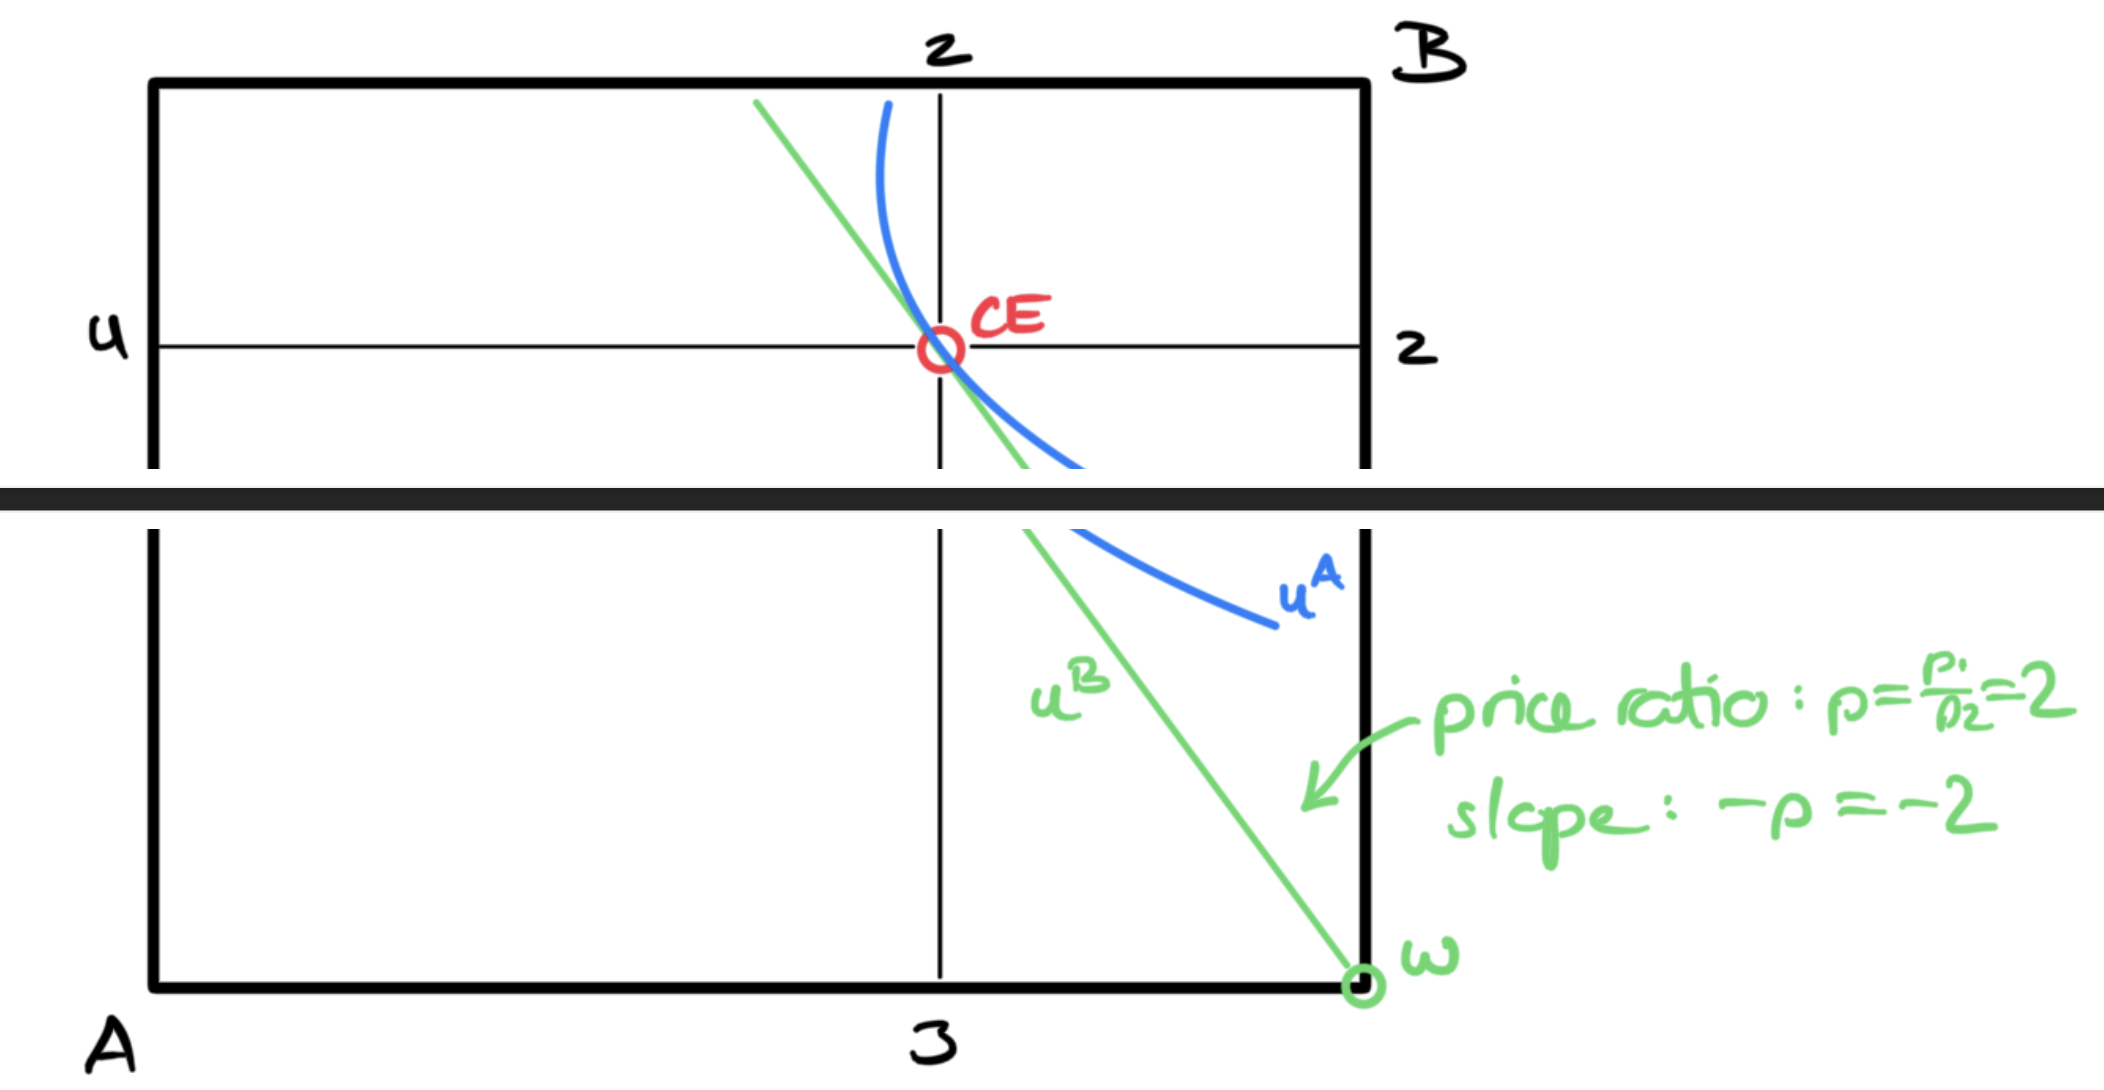
\includegraphics[width=0.75\linewidth]{images/2012_13_edgeworth_box.png}
    \caption{The vertical bar is not part of the figure. The figure was drawn on an iPad and the export created the line. Ignore it.}
\end{figure}
}
{\item 
Agent A cannot influence $x_2^B$. Thus, her FOC does not change: her behaviour is the same. The behavior of agent $B$ does not change as well. Thus, the CE remains the same.
But this CE does not need to be PE anymore, reason being that $X_2^B$ is on externality for A. Incomplete markets lead to inefficient CE allocations.
}
{\item 
\underline{type C:}
Under autarky there's no trade as consumers are identical. Free trade can only lead to a utility increase (or it stays the same) by voluntarity of trade.

\underline{type C:}
If the greater total endowment of good 2 in the economy increases $p$. then A profits as a seller of good 1 .
If price remains at $p=2$, there is no impact.

\underline{type B:}
If $p>2$, $B$ will not sell anything of good 2, and try to buy more of it (which she cannot).
she can't). Then $\left(u^B\right)^{j\text{FT}}=6=\left(u^B\right)^{\text{aut}}$. it $p=2$, also $\left(u^B\right)^{j\text{FT}}=6=\left(u^B\right)^{\text{aut}}$.
}

\subsubsection*{Exercise 2}

Convexity is not needed, but LNS is. Convexity is only needed for the SWT. If LNS is violated, we can immediately construct a counterexample with $L=H=2$:

Although CE exists, we could move south-west to increase B's utility without hurting A.

\begin{figure}[htp!]
    \centering
    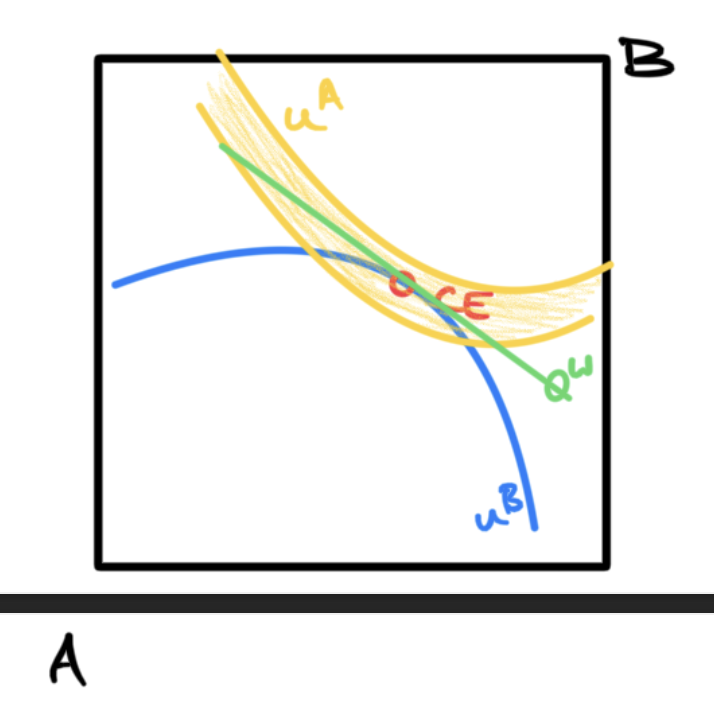
\includegraphics[width=0.75\linewidth]{images/2012_13_counterexample.png}
    \caption{The vertical bar is not part of the figure. The figure was drawn on an iPad and the export created the line. Ignore it.}
\end{figure}

\subsubsection*{Exercise 3}
\begin{enumerate}[label=(\alph*)]
{\item 
\begin{align*}
    w^1=(3,2) \quad w^2=(2,6)
\end{align*}

PE: equalize MRS across consumers.

\begin{align*}
    M R S^1=\frac{\pi(1) \frac{1}{x^{1}(1)}}{\pi(2) \frac{1}{x^1(2)}} 
    &\stackrel{!}{=} M R S^2=\frac{\pi(1) \frac{1}{x^2(1)}}{\pi(2) \frac{1}{x^2(2)}} \\
    \frac{x^{1}(2)}{x^{1}(1)} & =\frac{x^2(2)}{x^2(1)}
\end{align*}

Apply market clearing conditions:

\begin{align*}
    x^2(2) &= 8-x^{1}(2) \\
    x^2(1) &= 5-x^{1}(1)
\end{align*}

Thus: 

\begin{align*}
    \frac{x^{1}(2)}{x^{1}(1)} & =\frac{8-x^{1}(2)}{5-x^{1}(1)} \\
    \frac{8}{x^{1}(2)}-1 & =\frac{5}{x^{1}(1)}-1 \\
    x^{1}(2) & =\frac{8}{5} x^{1}(1)
\end{align*}

\begin{figure}[htp!]
    \centering
    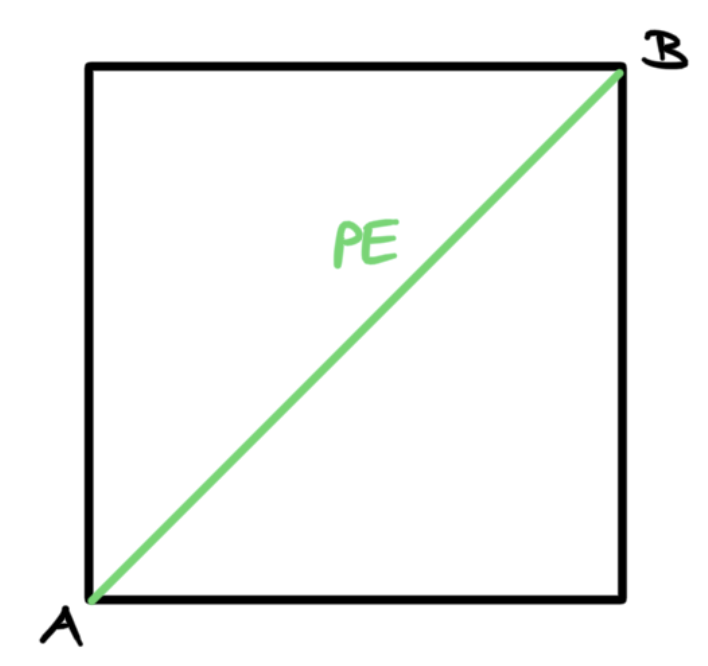
\includegraphics[width=0.5\linewidth]{images/2012_13_PE.png}
\end{figure}
}
{\item 
\underline{consumer h:}

\begin{align*}
    & \max _{x^h} \pi(1) \ln \left(x^h(1)\right)+\pi(2) \ln \left(x^h(2)\right) \\
    & \text { s.t. } \quad p(1)\left(x^h(1)-w^h(1)\right)+p(2)\left(x^h(2)-w^h(2)\right)=0
\end{align*}

The FOCs are

\begin{align*}
& \frac{\pi(1)}{x^h(1)}-\lambda p(1)=0 \\
& \frac{\pi(2)}{x^h(2)}-\lambda p(2)=0 \\
\Longrightarrow\quad &\frac{p(1)}{p(2)}=\frac{\pi(1)}{\pi(2)} \frac{x^h(2)}{x^h(1)} \tag{I}
\end{align*}

Equation (I) describes the relationship of prices and state probabilities. With identical beliefs, we have $\frac{x^{1}(2)}{x^{1}(1)}=\frac{x^2(2)}{x^2(1)}$, ie. PE and thus

\begin{align*}
    \frac{p(1)}{p(2)}=\frac{\pi(1)}{\pi(2)} \frac{8}{5}
\end{align*}

Therefore, in our case we find that $\frac{p(1)}{p(2)}>\frac{\pi(1)}{\pi(2)}$ because total endowment in state 1 is higher than in state 2. If there was greater total endowment in state 1, the inequality sign would switch to $<$. 
}
\end{enumerate}


\end{enumerate}
}
\newpage

\end{document}
